\section{Results}

\begin{table*}[t]
    \centering
    \small
    \resizebox{1\linewidth}{!}{
        \begin{tabular}{lcrr||c|lll||c|lll}
            \toprule
            \multicolumn{4}{c||}{\textbf{Model Information}} 
            & \multicolumn{4}{c||}{\textbf{MLP - Accuracy}} 
            & \multicolumn{4}{c}{\textbf{LSTM - Accuracy}} \\
            \cmidrule(lr){1-4} \cmidrule(lr){5-8} \cmidrule(lr){9-12}
            Backbone & Type & \#Params & \#Frames (Seconds)
            & Overall Accuracy & Brushing Class & Reading Class & Climbing Class 
            & Overall Accuracy & Brushing Class & Reading Class & Climbing Class \\
            \midrule
            yolo & By Frame & 2.9M & 8 (0.32) & 65.84\% ± 3.93 & 33.63\% ± 8.67 & 72.81\% ± 7.96 & 78.87\% ± 6.49 & 70.61\% ± 3.62 & 54.79\% ± 20.18 & 75.30\% ± 9.07 & 80.23\% ± 3.05 \\
            dino & By Frame & 22.1M & 8 (0.32) & 80.53\% ± 5.02 & 51.41\% ± 21.74 & 84.98\% ± 4.91 & 90.68\% ± 4.32 & 82.64\% ± 3.15 & 70.98\% ± 4.63 & 82.68\% ± 7.93 & \textbf{92.76}\% ± 3.45 \\
            clip & By Frame & 151.3M & 8 (0.32) & 77.08\% ± 1.88 & 48.76\% ± 16.31 & 77.66\% ± 9.70 & 91.05\% ± 3.56 & 78.72\% ± 3.04 & 58.30\% ± 10.55 & 85.84\% ± 5.69 & 89.55\% ± 5.02 \\
            \midrule
            r3d & By Segment & 31.6M & 8 (0.32) & 84.15\% ± 4.59 & 63.14\% ± 19.01 & 86.92\% ± 3.79 & \textbf{92.22}\% ± 2.87 & \textbf{86.80}\% ± 3.50 & 83.46\% ± 4.18 & 87.06\% ± 3.67 & 89.71\% ± 5.64 \\
            i3d & By Segment & 12.7M & 16 (0.64) & 77.61\% ± 7.96 & 56.66\% ± 13.86 & 77.69\% ± 6.42 & 89.88\% ± 5.74 & 79.38\% ± 5.68 & 71.62\% ± 5.64 & 75.79\% ± 16.07 & 89.04\% ± 6.34 \\
            x3d-xs & By Segment & 3.0M & 4 (0.16) & 81.64\% ± 3.76 & 62.65\% ± 12.53 & 82.48\% ± 6.19 & 90.58\% ± 4.65 & 84.90\% ± 2.68 & 81.50\% ± 4.99 & 83.73\% ± 3.82 & 89.80\% ± 3.95 \\
            x3d-s & By Segment & 3.0M & 16 (0.64) & 84.89\% ± 4.90 & 69.96\% ± 14.65 & \textbf{88.83}\% ± 3.71 & 88.48\% ± 5.21 & 85.97\% ± 2.84 & \textbf{84.88}\% ± 5.92 & 82.70\% ± 4.17 & 89.97\% ± 5.78 \\
            x3d-m & By Segment & 3.0M & 16 (0.64) & \textbf{85.39}\% ± 4.16 & \textbf{72.03}\% ± 16.10 & 87.13\% ± 4.09 & 90.50\% ± 4.55 & 85.65\% ± 2.22 & 84.00\% ± 9.41 & 84.45\% ± 6.60 & 89.16\% ± 2.85 \\
            x3d-l & By Segment & 5.3M & 16 (0.64) & 84.79\% ± 4.04 & 69.36\% ± 16.20 & 86.55\% ± 3.81 & 91.35\% ± 2.53 & 85.46\% ± 1.47 & 84.26\% ± 6.07 & 84.41\% ± 8.37 & 87.82\% ± 4.21 \\
            s3d-k & By Segment & 7.9M & 16 (0.64) & 78.38\% ± 5.21 & 57.96\% ± 11.23 & 77.66\% ± 11.26 & 89.65\% ± 2.84 & 78.57\% ± 4.06 & 77.65\% ± 4.85 & 73.37\% ± 5.84 & 84.53\% ± 7.77 \\
            s3d-h & By Segment & 7.9M & 16 (0.64) & 59.52\% ± 8.90 & 00.00\% ± 00.00 & 78.96\% ± 7.35 & 76.79\% ± 15.54 & 43.25\% ± 4.74 & 23.56\% ± 34.56 & 42.93\% ± 29.85 & 58.29\% ± 43.94 \\
            slowfast & By Segment & 33.6M & 32 (1.28) & 84.06\% ± 2.94 & 70.79\% ± 12.22 & 85.00\% ± 2.27 & 90.47\% ± 1.33 & 85.16\% ± 1.80 & 79.18\% ± 7.60 & \textbf{88.54}\% ± 6.68 & 87.82\% ± 3.96 \\
            vivit & By Segment & 88.6M & 32 (1.28) & 77.65\% ± 5.19 & 45.44\% ± 14.48 & 81.71\% ± 8.27 & 90.93\% ± 5.70 & 81.46\% ± 2.21 & 72.71\% ± 9.25 & 82.14\% ± 6.72 & 87.14\% ± 5.72 \\
            \bottomrule
        \end{tabular}
    }
    \vspace{-2ex}
    \centering
    \caption{Models Performance Results.}
    \paragraph{
        The duration in seconds is relative to a 25 FPS video. Note that the X3D  models have the same number of parameters but the FLOPs increase between each member of the family.
    }
    \label{table:training-results}
\end{table*}
    

\begin{figure*}[!htb]
    \centering
    \begin{minipage}{0.48\textwidth}
        \centering
        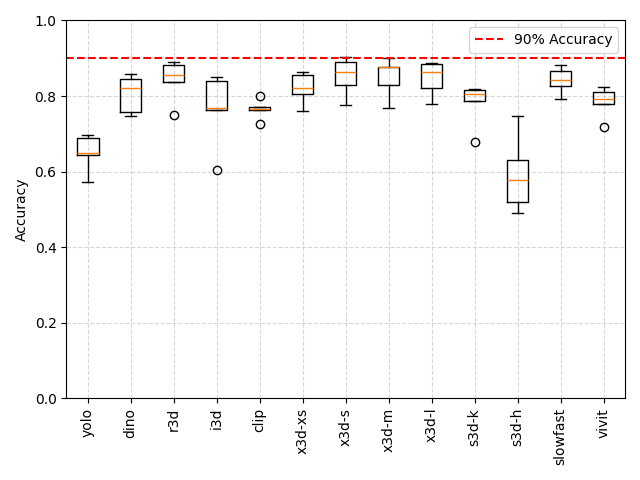
\includegraphics[width=0.45\textwidth]{../../assets/figures/mlp.training-results.boxplot.png}
        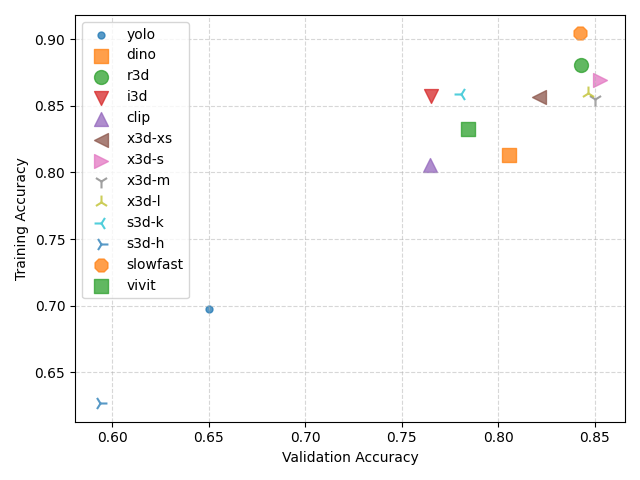
\includegraphics[width=0.45\textwidth]{../../assets/figures/mlp.training-results.scatter.png}
        \caption{MLP Model Training Results}
        \label{fig:mlp-training-results}
    \end{minipage}
    \hfill
    \begin{minipage}{0.48\textwidth}
        \centering
        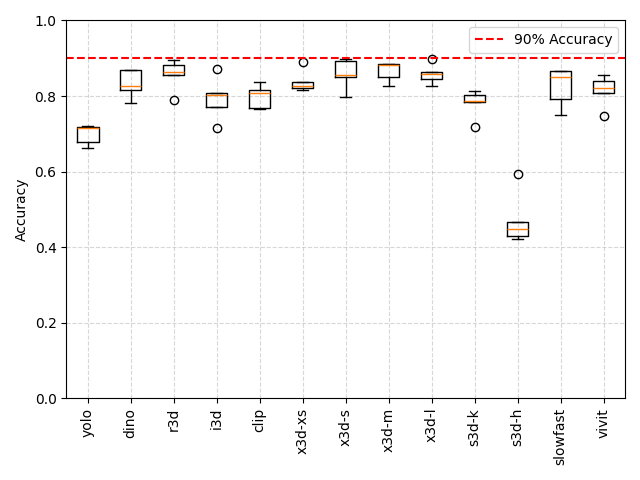
\includegraphics[width=0.45\textwidth]{../../assets/figures/lstm.training-results.boxplot.png}
        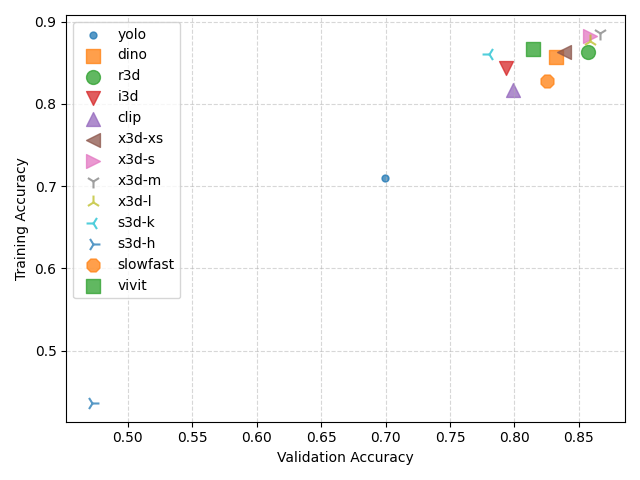
\includegraphics[width=0.45\textwidth]{../../assets/figures/lstm.training-results.scatter.png}
        \caption{LSTM Model Training Results}
        \label{fig:lstm-training-results}
    \end{minipage}
\end{figure*}

\subsection{Performance Analysis}
Table~\ref{tab:model-performance} presents the classification accuracy of various backbone architectures combined with either MLP or LSTM classifiers for bouldering video segmentation. The results reveal several interesting patterns that provide insights into the effectiveness of different approaches for this specific task.

\subsubsection{Temporal vs. Frame-based Feature Extraction}
Our experiments demonstrate a clear advantage for models that incorporate temporal information through segment-level processing. As shown in Table~\ref{tab:model-performance}, segment-based models consistently outperform frame-based models, with the top-performing models (X3D family) all utilizing temporal information. The X3D-S model achieves 85.28\% accuracy with an MLP classifier, while X3D-M reaches 86.61\% accuracy when combined with an LSTM. This pattern aligns with the intuitive understanding that climbing actions involve temporal dynamics that cannot be fully captured by analyzing individual frames or segments in isolation.

\subsubsection{Analysis of Underperforming Models}
Two backbone architectures exhibit notably lower performance compared to others:

\noindent\textbf{YOLO-based Skeleton Features.}
The YOLO-based approach, which extracts skeletal key points, achieves only 65.01\% accuracy with MLP and 69.94\% with LSTM. This underperformance can be attributed to the similarity in climber movement dynamics across different action categories. For instance, the speed and pattern of movement during observing, brushing, and climbing activities may exhibit similar skeletal motion signatures despite being semantically distinct. A potential improvement would be to incorporate absolute spatial positions rather than positions relative to the climber's center of mass. However, this approach would introduce camera position dependency, potentially reducing generalizability across different recording setups.

\noindent\textbf{S3D with HowTo100M Pre-training.}
The S3D model pre-trained on HowTo100M (S3D-H) shows particularly poor performance (59.37\% with MLP, 47.19\% with LSTM). This can be explained by the nature of the pre-training dataset, which consists primarily of instructional videos featuring fine-grained hand manipulations and subtle movements. The same architecture pre-trained on the Kinetics dataset (S3D-K), which contains more diverse and dynamic whole-body activities, performs substantially better (78.08\% with MLP, 78.04\% with LSTM). This significant performance gap highlights the critical importance of selecting appropriate pre-training datasets that align with the target domain's action characteristics.

\subsubsection{Model Complexity and Performance}
Interestingly, our experiments reveal that larger models do not necessarily yield better performance for this task. The X3D-S model (3.0M parameters) outperforms the larger X3D-L variant (5.3M parameters) when using an MLP classifier. Similarly, the relatively lightweight R3D backbone (31.6M parameters) achieves better results to much larger models such as CLIP (151.3M parameters) and ViViT (88.6M parameters). This suggests that for our specific dataset size and task complexity, model architecture design is more important than raw parameter count. The X3D family, designed specifically for efficient video understanding, demonstrates excellent performance-to-parameter ratios across all variants.

\subsubsection{Temporal Modeling with LSTM}
When comparing MLP and LSTM classifiers, we observe that LSTM generally provides modest improvements across most backbones. For instance, DINO shows a 2.62 percentage point improvement when switching from MLP to LSTM. However, this pattern is not universal—SlowFast actually performs 1.73 percentage points worse with LSTM compared to MLP. The inconsistent benefits of additional temporal modeling through LSTM may be due to our dataset size constraints, as larger datasets typically show more significant improvements from temporal modeling, as demonstrated in prior work \cite{example-paper-doing-temporal-modeling}.
\todo[inline]{Cite the Action Clip Paper which uses LSTMS on the CLIP features.}

Beyond improvements in accuracy, we also observe a reduction in variance across multiple runs when using LSTM classifiers. For example, the X3D-M model shows a standard deviation of 4.75\% with MLP but only 2.32\% with LSTM, representing a nearly 50\% reduction in variance. This increased stability is a significant advantage in practical applications, as it indicates more reliable and consistent performance across different climbing sessions and environmental conditions.

\subsection{Practical Implications}
Based on our experimental results, we can draw several conclusions to guide model selection for practical bouldering video segmentation applications:

\noindent\textbf{For accuracy-critical applications.}
The X3D-M with LSTM classifier provides the highest overall accuracy (86.61\%) and represents the best choice when classification performance is the primary concern.
    
\noindent\textbf{For resource-constrained environments.}
The X3D-XS with MLP classifier offers an excellent balance between accuracy (82.11\%) and computational efficiency, utilizing only 3.0M parameters. And this model provide the best trade-off between speed and accuracy.
    
These findings provide valuable insights for climbing gym operators, sports coaches, and performance analysts working with climbing videos. For coaches analyzing technique, the highest accuracy models would better distinguish between different climbing phases, while training facilities with limited computing resources could implement the lighter models for real-time feedback systems. The ability to reliably segment climbing activities enables more targeted training programs and better performance assessment for climbers at all levels.